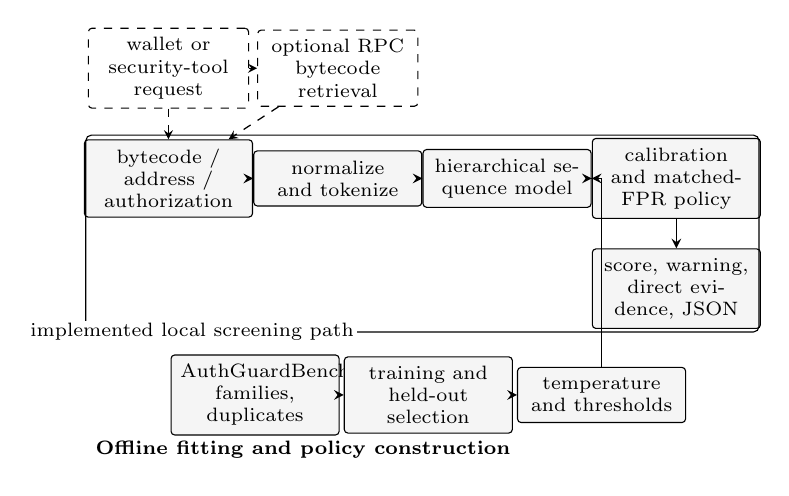
\begin{tikzpicture}[
  font=\scriptsize,
  box/.style={draw, rounded corners=1.3pt, minimum height=7mm, text width=19mm,
              align=center, fill=gray!8},
  ext/.style={draw, dashed, rounded corners=1.3pt, minimum height=7mm, text width=18mm,
              align=center},
  flow/.style={->, >=stealth, line width=.55pt},
  context/.style={->, >=stealth, dashed, line width=.45pt}
]
  \node[ext] (wallet) at (-3.2,2.0) {wallet or security-tool request};
  \node[ext] (rpc) at (-1.05,2.0) {optional RPC bytecode retrieval};
  \node[box] (input) at (-3.2,.6) {bytecode / address / authorization};
  \node[box] (token) at (-1.05,.6) {normalize and tokenize};
  \node[box] (model) at (1.10,.6) {hierarchical sequence model};
  \node[box] (policy) at (3.25,.6) {calibration and matched-FPR policy};
  \node[box] (output) at (3.25,-.8) {score, warning, direct evidence, JSON};
  \draw[context] (wallet) -- (rpc);
  \draw[context] (wallet) -- (input);
  \draw[context] (rpc) -- (input);
  \draw[flow] (input) -- (token);
  \draw[flow] (token) -- (model);
  \draw[flow] (model) -- (policy);
  \draw[flow] (policy) -- (output);

  \node[box] (bench) at (-2.10,-2.15) {AuthGuardBench, families, duplicates};
  \node[box] (train) at (.10,-2.15) {training and held-out selection};
  \node[box] (cal) at (2.30,-2.15) {temperature and thresholds};
  \draw[flow] (bench) -- (train);
  \draw[flow] (train) -- (cal);
  \draw[flow] (cal.north) |- (policy.west);
  \draw[rounded corners=2pt] (-4.25,-1.35) rectangle (4.30,1.15);
  \node[fill=white, inner sep=1pt] at (-2.9,-1.35) {implemented local screening path};
  \node[anchor=west] at (-4.25,-2.85) {\textbf{Offline fitting and policy construction}};
\end{tikzpicture}

